\chapter{Introduction}
\label{chapter-introduction}

This thesis describes advances in theorem proving in first-order intuitionistic
logic.  We show that the \emph{polarized inverse method}, a focused, bottom-up
proof search procedure, combined with \emph{constraints} yields an efficient,
general, and practical tool for some kinds of intuitionistic automated
reasoning.To provide evidence for our claim of efficiency, we built a framework
based on the polarized inverse method with constraints called \emph{Imogen}.
Imogen is competitive with the best existing theorem provers in pure
propositional logic.  It is the best performing implementation for pure
first-order logic.  To provide evidence for our claim of generality, we use
Imogen to build theorem provers for intuitionistic modal logic, linear logic,
and ordered logic.  To provide evidence for our claim to practicality, we used
the framework to build useful tools for analyzing networking and authorization
in the Amazon Web Services (AWS) cloud.

\subsubsection*{Constraints}

The main contribution of the thesis is the use of \emph{constraint domains}
together with the polarized inverse method. Pure first-order logic treats
function symbols as \emph{uninterpreted}; any facts about the symbols are
explicit in the formula.  Constraint domains make the behavior of some function
symbols implicit.  For example, if we are reasoning about integers, the ``+''
symbol can be interpreted as addition without explicitly giving axioms defining
addition in the formula itself.  As another example, the domain of bit-vectors
are particularly useful in applications to computer networks.  For example,
given three 32-bit vectors, the first ($\Ip$) representing an IP address, the
second two representing the two components of a CIDR range ($\Base$, $\Mask$),
the following formula defines a predicate $\Matches$, which indicates that the
IP belongs to the CIDR range:

\[
\All\Ip, \Base,\ \Mask: \BV_{32}.\
  \Matches(\Ip, \Base, \Mask) \Iff \Ip \BvAnd \Mask = \Base\BvAnd\Mask
\]

\noindent
Here the domain consists of the sort $\BV_{32}$ of bit-vectors of length 32,
the bitwise ``and'' operator (\&), and equality on bit-vectors.  An IP address
$\Ip$ matches a CIDR range if the bitwise ``and'' of $\Ip$ with the subnet
mask $\Mask$ is identical to the CIDR start address $\Ip$ ``and''-ed with
$\Mask$.  For example, we would expect the following to be provable:

\[
\begin{array}{l}
  \Matches(10.0.10.10, 10.0.0.0, 255.255.0.0)
  \\[5pt]
  \Not\Matches(10.1.10.10, 10.0.0.0, 255.255.0.0)
  \\[5pt]
  \All\Ip, \Base: \BV_{32}.\
  \Matches(\Ip, \Base, 255.255.255.255) \Imp \Ip = \Base
\end{array}
\]

\noindent
We will use constraint like these extensively in our case
study where we apply these methods to analyzing networks in the
AWS cloud in Chapter~\ref{chapter-aws}.

Constraints do not change what is expressible in first-order logic.  Any formula
expressible with constraints is expressible without them.  Continuing with the
bit-vector example, we can first encode bit-vectors of length 32 as functions
$\Set{0, \ldots, 31} \to \Set{0, 1}$.  Then we can define

\[
(f\,\&\,g)(N) \Eqdef f(N)\,\&\,g(N)
\]

\noindent where the second $\&$ is the boolean
``and''.  Equality would be defined extensionally on bit-vectors;
\[f = g \Iff \All n\in\Set{0,\ldots, 31}.\ f(n) = g(n)\] where the second $=$ is
equality on the set $\Set{0,1}$.  Indeed, some classical first-order theorem
provers take this approach, since it does not require changing the
implementation.  However, we show that, at least for the
inverse method, using constraints is a far more efficient approach to
domain-specific reasoning.

\subsubsection*{Why Intuitionistic Logic?}

This work exclusively studies \emph{intuitionistic} logics.  Intuitionistic
logic has been largely ignored by the applied theorem proving community.  There
are good reasons for this; it's much more difficult to prove theorems in
intuitionistic logic than in classical logic.  The propositional case, for
example, is PSPACE-complete vs. NP-complete for classical logic.  Classical
logic has beautiful normal forms that lead naturally to simple algorithms like
DPLL that have in recent years solved astonishingly large SAT problems, and are
applied all over industry, particularly in hardware and software verification.
First-order classical logic has even nicer normal forms, due to tricks like
Skolemization, that lead again to efficient algorithms like resolution and
paramodulation.  In contrast, but for to our knowledge there are no intuitionistic
theorem provers in industrial use is there are no existing theorem provers that
efficiently handle equality in intuitionistic logic.   not necessarily
clear what you gain from
intuitionism.

In our view, the one way in which classical theorem provers are lacking is in
the evidence they give for the truth of a proposition.  Theorem proving in
classical logic is generally based on refutation; the formula is negated, and
the resulting formula is proved unsatisfiable, which indirectly implies the
original proposition is true.  While we do not doubt the consistency of
the logic, the generated resolution proofs, for example, only show that a
contradiction was obtained, and it is difficult to mine such a proof for
human-digestible justification.

In contrast, intuitionistic logic has a beautiful proof theory that corresponds
to a simple programming language.  As a result, it is possible to generate
understandable evidence that demonstrates the truth of a proposition.  For some
applications, knowing \emph{why} a proposition is true as important as knowing
\emph{that} it is true (cf. Chapter~\ref{chapter-aws}).  For a simple example,
consider the SMT-LIB program shown in Figure~\ref{figure.z3-path}.  It defines
the the type of nodes with three elements $a, b, c$ and predicates \textsf{edge}
and \textsf{path}.  Edges are atomic.  A path is either an edge, or a
combination of two paths that share an endpoint.  Then it defines edges between
$a, b$ and $b, c$.  Finally, it asks whether there's a path between $a$ and $c$.
Imogen Z3, an industrial-strength SMT solver finds the 3700 byte refutation
proof shown in Figure~\ref{figure.z3-proof}.  The equivalent constructive proof
in Imogen is

\[
\begin{array}{rl}
  &\lambda H1: \forall x\ y.\ edge(x, y) \Imp path(x, y). \\
  &\lambda H2: \forall x\ y\ z.\ path(x, y) \Imp path(y, z) \Imp path(x, z).\\
  &\lambda H3: edge(a, b). \\
  &\lambda H4: edge(b, c). \\
  &\hspace{1em}  H2\ a\ b\ c\ (H1\ a\ b\ H3)\ (H1\ b\ c\ H4)
\end{array}
\]

\begin{figure}
  \VerbatimInput[frame=lines, fontsize=\footnotesize]{figs/z3-path.smt2}
  \caption{Paths in a graph}
  \label{figure.z3-path}
\end{figure}

\begin{figure}
  \VerbatimInput[frame=lines, fontsize=\tiny]{figs/z3-proof.txt}
\caption{Z3 Proof}
\label{figure.z3-proof}
\end{figure}

Our intention is not to single out Z3 as a poor example of proof objects, but to
emphasize that classical refutation proofs have less useful information than
intuitionistic proofs.  While this fact has been a matter of philosophical
discourse for over well over a century, its \emph{usefulness} in building
useful analysis tools has been under-appreciated.  For example, constructive
proofs like the one shown above can be processed into a form
that is helpful in debugging, e.g. complicated authorization policies.

\section{Overview of the Thesis}

\begin{quote}
\textbf{Thesis Statement:} The polarized inverse method, augmented with
general constraint domains, is an effective and practical method of
automated reasoning in intuitionistic logics.
\end{quote}

To begin, in Chapter~\ref{chapter-prop} we will describe the polarized inverse
method in detail for intuitionistic propositional logic.  While the
propositional fragment lacks both constraints and quantifiers, it demonstrates
the primary theorem proving algorithm in its simplest form.  Besides showing the
calculus and proving soundness and completeness, we show a number of
optimizations that make our implementation competitive with the best existing
solvers.  Foremost among the optimizations are a series of ``polarity
disciplines'' that we call \emph{logical optimizations}.  The defining feature
of logical optimizations is that they operate only on the input formula, and are
independent of a given inverse method implementation.

In Chapter~\ref{chapter-fol} we extend the propositional prover with first-order
quantifiers.  The completeness theorem is more complicated, but similar in
spirit.  We demonstrate the effectiveness of our base method on problems from
the TPTP library.  Our implementation solves more first-order problems than any
existing prover for intuitionistic logic.

Chapter~\ref{chapter-constraints} is the main theoretical contribution of the
thesis.  We describe how to add constraints to the polarized inverse method and
prove soundness and completeness results.  The proofs are parameterized on a
given constraint domain.  We show that the domain needs only a small number of
reasonable properties (transitivity of entailment, for example) for the theorems
to work.  To finish the chapter we add bitvector and finite domain constraints
to the first-order prover from Chapter~\ref{chapter-fol}.

Chapter~\ref{chapter-aws} is a case study in using our method on a real-world
problem encountered by the author in industry: verifying properties of
cloud networking on Amazon Web Services (AWS).

Chatper~\ref{chapter-modal} shows how to apply constraints to obtain theorem
provers for some intuitionistic modal logics.

Chatper~\ref{chapter-sub}, joint work with Jason Reed, shows how to apply
constraints to obtain theorem provers for linear and ordered logic.

\begin{figure}[H]
  \begin{center}
    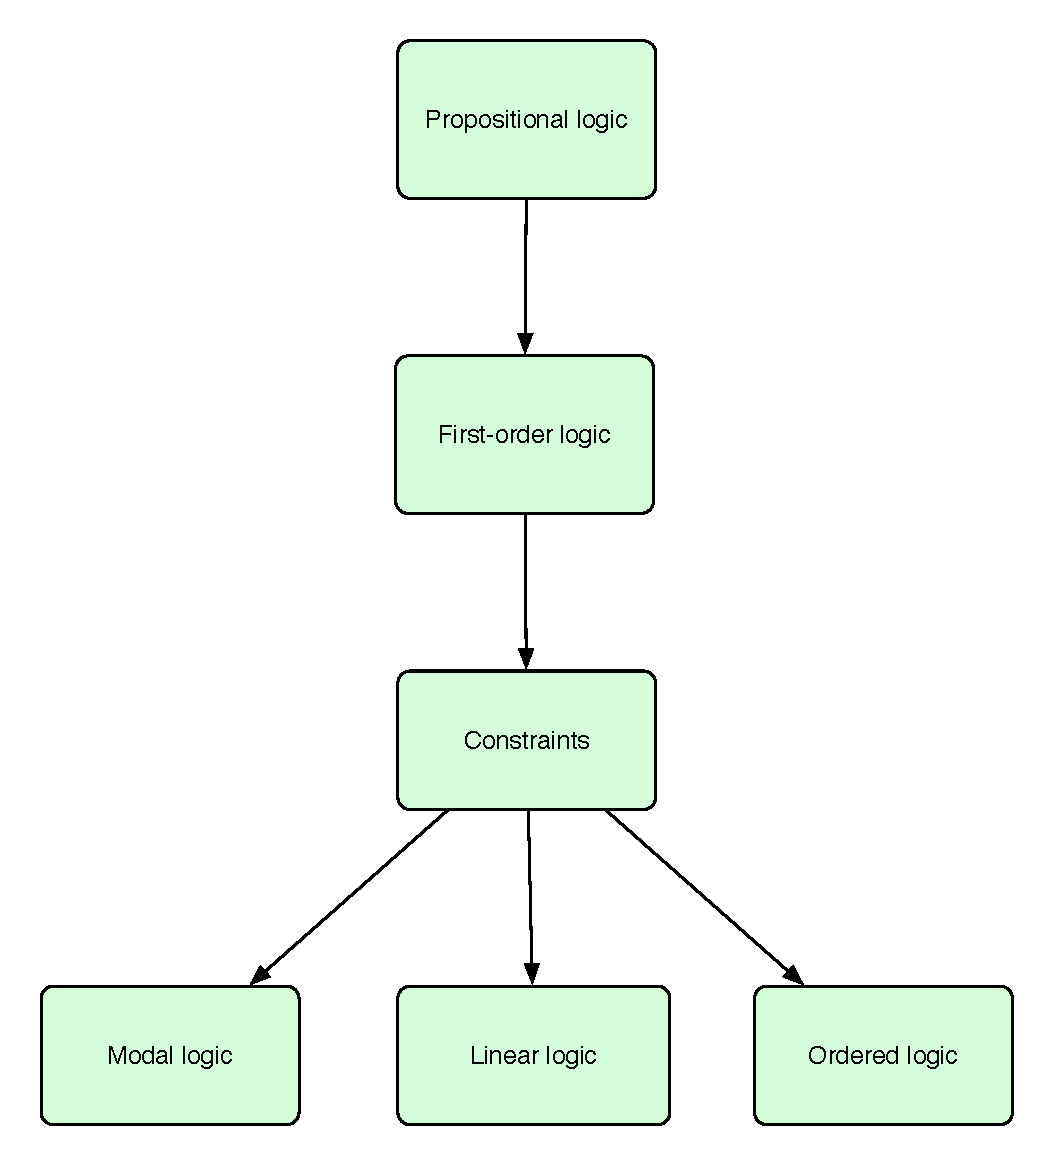
\includegraphics[scale=0.50]{figs/logics.eps}
  \end{center}
  \caption{Logics}
  \label{figure.logics}
\end{figure}

\section{Related work}

Constraints are nothing new in the literature.  Constraint logic programming and
satisfiability modulo theories (SMT) are devoted to the study of the interplay
between general logical reasoning and reasoning in constraint domains.  This
research differs from existing work in a couple of ways.  First, we are
considering full first-order intuitionistic logic as our base logic.  Constraint
logic programming remains, for all its improvements over Prolog's simple
operational semantics, a search and optimization procedure.  It can not be used
for general theorem-proving.  SMT comes closer, in that it combines solvers for
various constraint domains with classical first-order logic, though support for
arbitrary quantifier nesting is scant.  Vampire~\cite{Riazanov.1999.CADE} is the
best existing first-order classical theorem prover at the time of writing.  It
supports constraints by automatically adding (incomplete) axiomitizations of the
domains to input formulas.  Besides the obvious difference that Vampire is based
on classical logic, while our work deals with intuitionistic logic, we build
constraints into the core reasoning mechanism.


%%% Local Variables:
%%% mode: latex
%%% TeX-master: "thesis"
%%% End:
